\documentclass[12pt]{article}
\usepackage[margin=1in,letterpaper]{geometry}
\usepackage{amsmath}
\usepackage{subcaption}
\usepackage{mathrsfs} 
\usepackage{amsfonts}
\usepackage[titletoc,title]{appendix}
\usepackage{graphicx}
\usepackage{floatrow}
% Table float box with bottom caption, box width adjusted to content
\newfloatcommand{capbtabbox}{table}[][\FBwidth]
\usepackage{hyperref}
\hypersetup{
    colorlinks = true,
    citecolor={black},
    linkcolor={red}
}
\usepackage{titling}
\posttitle{\par\end{center}}
\setlength{\droptitle}{0pt}
\usepackage[numbers]{natbib}
\newcommand\citeay[1]{%
  \citeauthor{#1}~(\citeyear{#1})}

\begin{document}
\title{Crowd Segmentation Progress}
\author{\today}
\date{}
\vspace{-50pt}
\maketitle
\vspace{-70pt}
\section{Problem Formulation}
 The goal of quality evaluation is two-folds. Given N worker responses, find: 
 \begin{enumerate}
\item the quality of the bounding boxes (BB) drawn by worker 
\item the best proposed region for a given object in an image
 \end{enumerate}
\section{Key Assumptions and Intuitions}
\begin{enumerate}
\item In literature, there are scoring functions that require ``ground truth" and ones that are ``unsupervised". 
\item If a worker's response differs greatly from the ground truth, then work quality ($Q_w$) is low. 
\item If most of the workers' response differ greatly from ground truth for a particular image, then task difficulty ($D_t$) should be high. As a corollary, if the spread of the worker distribution ($J_i$) is large, then $D_t$ should also be high.
\end{enumerate}
To compute the latent quantities $Q_w$,$D_t$, we propose an iterative EM-like algorithm, where at every step, we assume that the ground truth bounding box ($BB_G$) is the current estimate of the maximum likelihood region. The maximum likelihood region is constructed by adding in sub-regions from a tile-graph. 
\section{Model}
\subsection{Definitions}

The model is inspired by the image-labelling model from \cite{MDWWelinder2010} with modifications for the segmentation task as follows:
\begin{itemize}
\item A task is defined by an object-image pair i : 
\begin{itemize}
\item $z_i$ is hidden variable that completely describes the ground truth BB from the image (e.g. set of all points in $BB_G$). $z_j$ is the BB drawn by worker j.
\item  $\phi_j$ is some descriptive image-related quantity extracted from worker BB $z_j$. This can either be a 1-D scalar aggregate or a multidimensional quantity. (e.g. boundary complexity of the image boundary) Sometimes, these summarization functions require a comparison against the ground truth $z_j$, so more generically we denote $\phi_j$ as $\phi_{ij}$
\item $J_i$ is the set of all workers j that annotated the object-image. 
\item $D_i$ is the task difficulty of object-image i. The $\phi_i$ image summary  of object i's ground truth BB $z_i$. The task difficulty is a dependent variable measuring how far off are most of the worker's responses ($z_j$) compared to $z_i$.  
\begin{equation}
D_i = \sum_{j\in J_i} dist(\phi_{ij},\phi_i)
\label{task_difficulty}
\end{equation}
\end{itemize}
\item We assume, by definition, that task difficulty is completely a result of the image itself and independent of any worker qualities. $q_{ij}$ is the quality of worker j for object i evaluated against $z_i$\footnote{We can also try to model user expertise separate from $q_{ij}$ which define only the vision-related quantities related to worker j's judgement on $\phi_{ij}$, but this is less important in salient, common-object segmentation.}.
\begin{equation}
q_{ij} = dist(\phi_{ij},\phi_i)
\label{worker_quality}
\end{equation}
\item Both the characteristics of the ground truth BB ($\phi_i$) and the worker's ability to segment the image ($q_j$) would determine how the worker would perceive the image($\phi_{ij}$) and the BB drawn by the worker ($z_{j}$) would look like.
\item To determine the quality of a worker ($q_j$), we can take some type of aggregate over all tasks performed by the workers. Averaging is a good aggregate functions because the number of tasks performed by each worker can vary a lot:
\begin{equation}
q_j = \frac{1}{\text{Total \# tasks by worker j}}\sum_i q_{ij}
\end{equation}
This direct technique to finding $q_j$ is used in the analysis in Sec.\ref{qi_analysis}.
%\item Finally, the characteristics of the BB drawn by worker i is just a summary of the BB drawn by worker i ($BB_i$)
\end{itemize}
\subsection{Inference}
\par The section above gives an empirical description of how work quality and image difficulty would be computed. However, in the inference process, we are interested in modelling image difficulty as a random variable. Simmilarly, the worker quality is also a random variable characterized by the worker's bias ($b_j$) and their consistency ($c_j$) across all tasks. Our hidden variables are the task difficulty for each image($\textbf{D}=\{D_i\}$) , true bounding box for the object ($\textbf{z}=\{z_i\}$) and the worker qualities ($\textbf{b}=\{b_j\}$,$\textbf{c}=\{c_j\}$) based on the worker bounding boxes ($\mathcal{L}=\{z_{ij}\}$) that we observe.

\begin{figure}[ht]
\centering
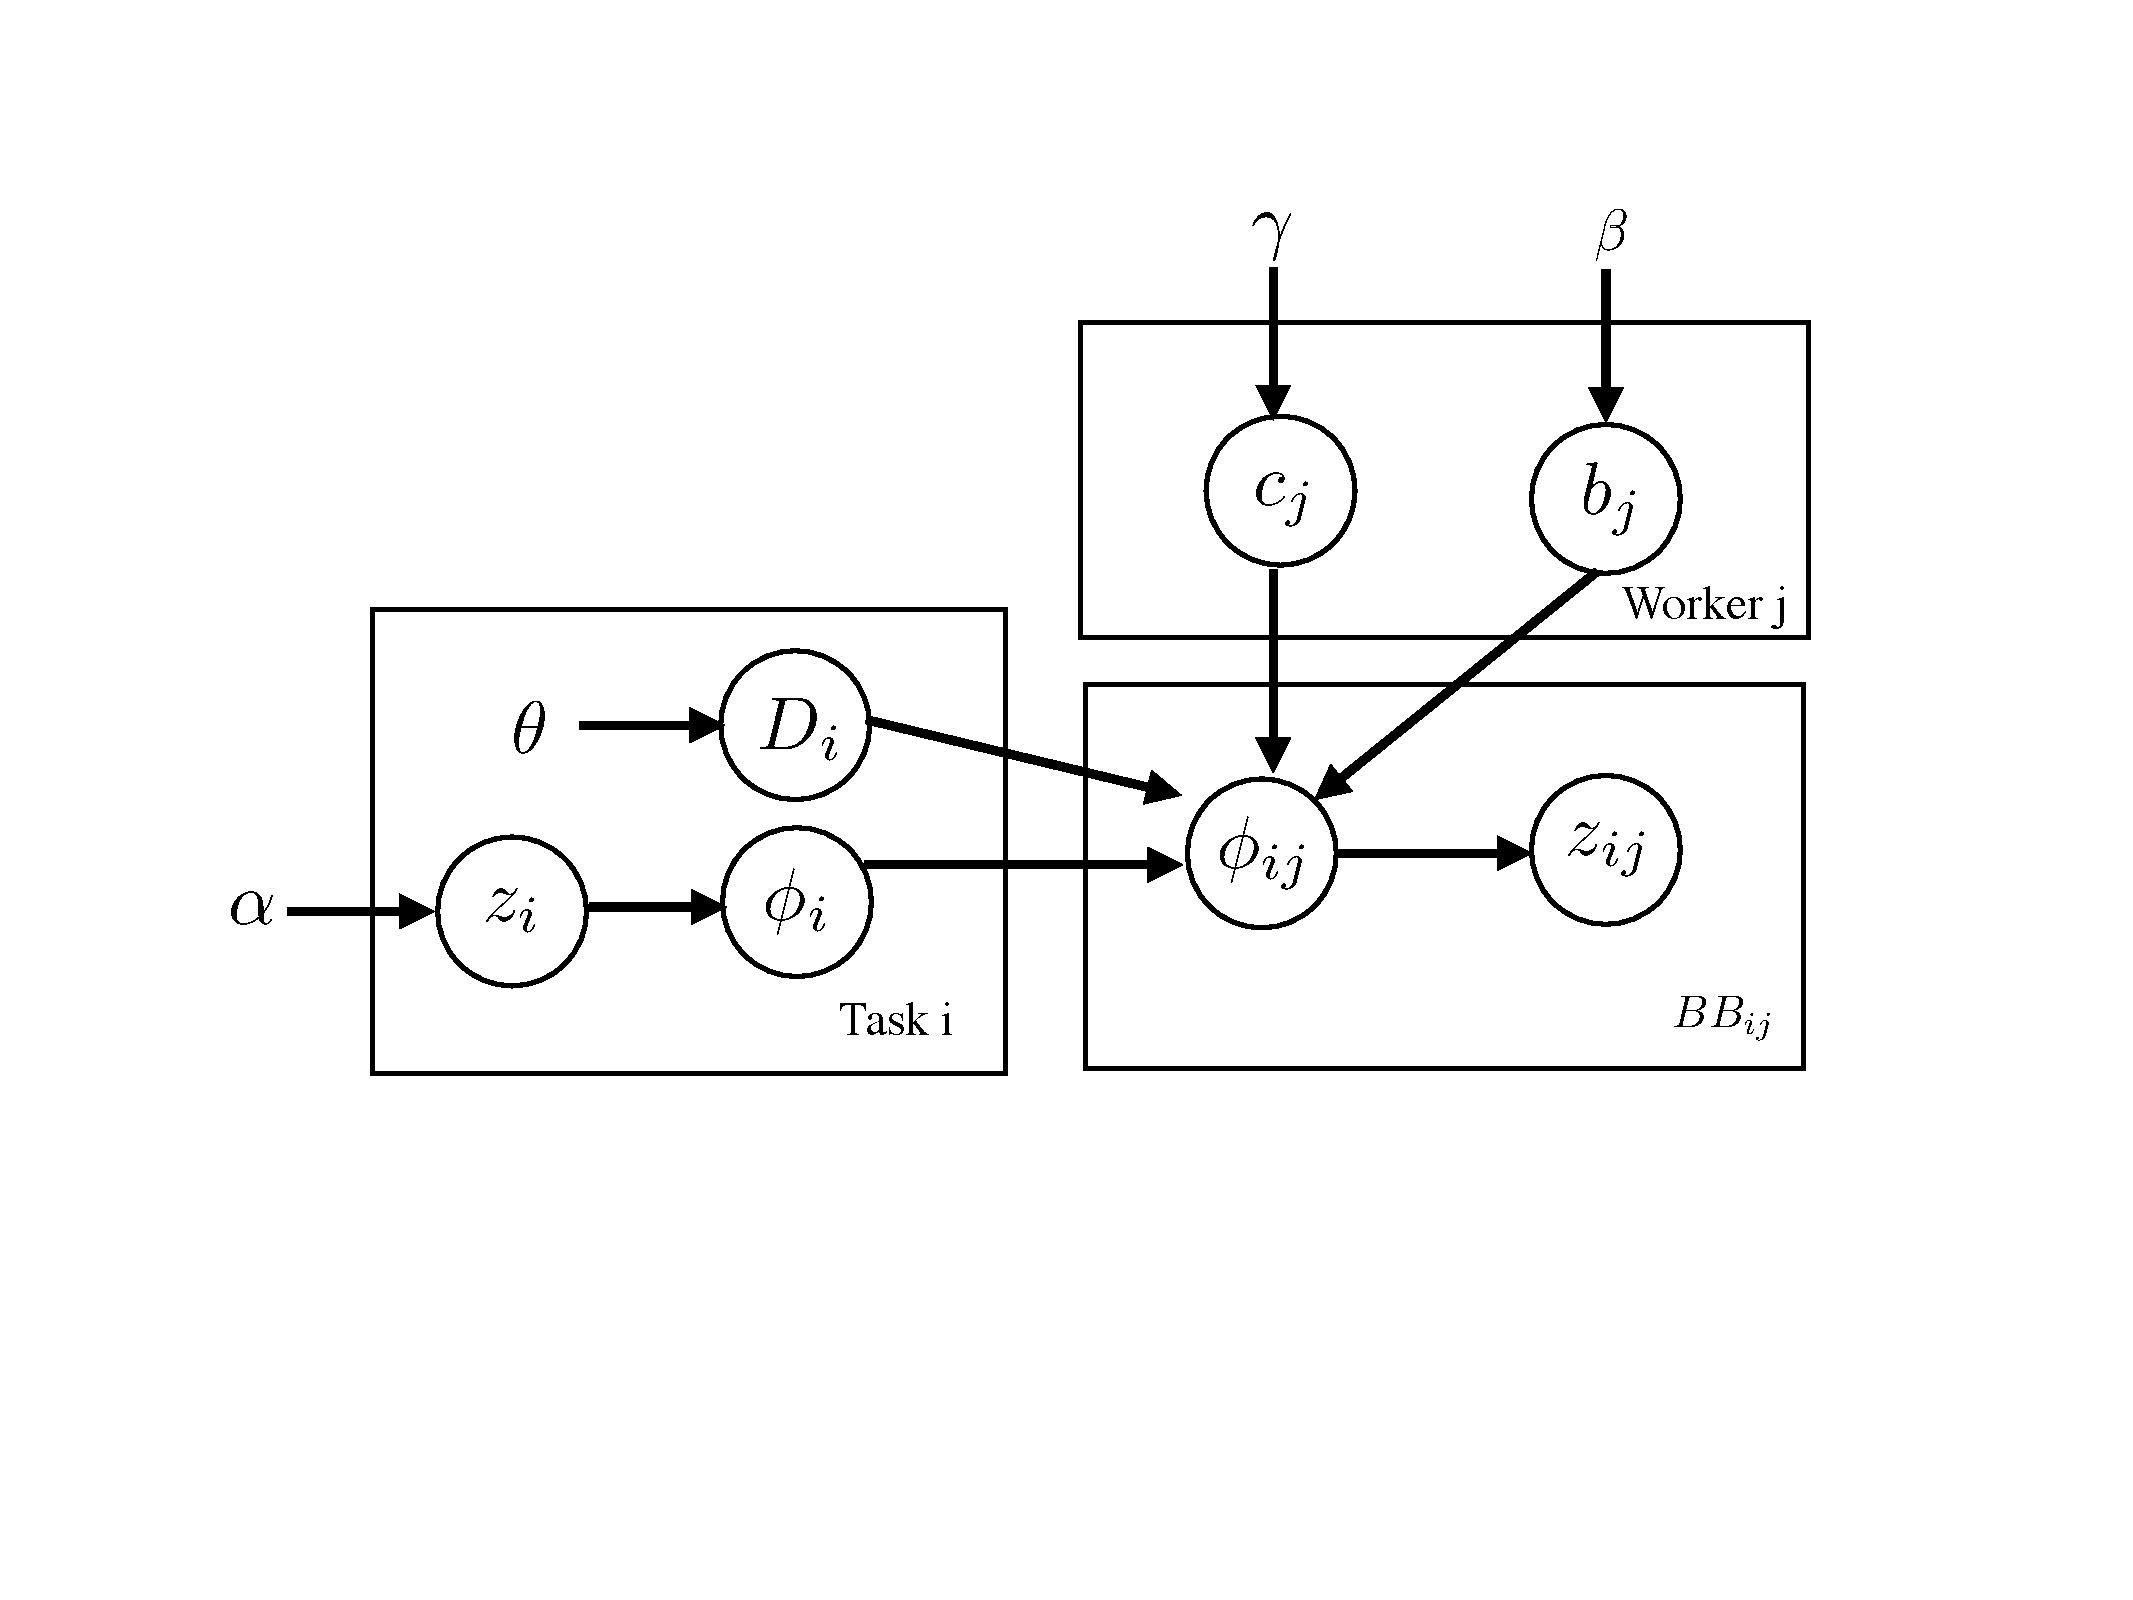
\includegraphics[trim=1cm 5cm 1cm 5cm,width=0.8\linewidth]{plots/generative_pgm2.pdf}
\caption{Proposed probabilistic graphical model for crowdsourcing image segmentation.}
\end{figure}
\par The joint probability distribution can be factored as:
\begin{equation}
p(\mathcal{L},\textbf{z},\textbf{q},\textbf{D}) = \prod_i \Big[p(z_i)p(D_i)p(\phi_i | z_i)\prod_{j\in J_i} p(\phi_{ij}|b_j,c_j,\phi_i,D_i)p(z_{ij}|\phi_{ij})\Big]\prod_j p(b_j) p(c_j) 
\end{equation}
The summarization process for worker bounding boxes ($\phi_{ij}\leftrightarrow z_{ij}$) is deterministic, since $\phi_{ij}=\Phi(z_i,z_j)$, so $p(\phi_i | z_i)=1$.
\begin{equation}
p(\mathcal{L},\textbf{z},\textbf{q},\textbf{D}) = \prod_i \Big[p(z_i)p(D_i)\prod_{j\in J_i} p(\phi_{ij}|b_j,c_j,\phi_i,D_i)\Big]\prod_j p(b_j) p(c_j) 
\end{equation}
The summary of worker bounding box is drawn from a normal distribution with variance of the distribution accounts for the task difficulty ($D_i$) and worker consistency($c_j$), scaled by constant coefficient $w_1,w_2$ to ensure appropriate weighting between the variances. This agrees with our intuition that in a distribution of image descriptions for all workers, the larger the spread means that the task is difficult or when the worker exhibits inconsistent behaviors. The distribution is centered around the worker-perceived ground truth summarization, which is obtained by shifting the complete summarization of ground truth $\phi_{ii}$\footnote{For $\Phi$ functions that don't require a comparison against ground truth (e.g. numPts), let $\phi_{ii}=0$. } (a constant) by a worker-dependent bias factor.
\begin{equation}
p(\phi_{ij}|b_j,c_j,\phi_i,D_i)=\mathcal{N}(\phi_{ij};\mu=\phi_{ii}-b_j, \sigma=\sqrt{w_1 D_i^2+w_2 c_j^2})
\end{equation}
The process for generating a bounding box $p(z_i)$ is a constant, so we can ignore this term. We put Gaussian priors ($\beta,\gamma,\theta$) on $\textbf{b},\textbf{c},\textbf{D}$ for the purpose of inference. The priors on $\textbf{b},\textbf{c},\textbf{D}$ is centered on the origin. The joint probability can be written as : 
\begin{equation}
p(\mathcal{L},\textbf{z},\textbf{q},\textbf{D}) = \prod_i \Big[p(D_i|\theta)\prod_{j\in J_i} \mathcal{N}(\phi_{ij};\mu, \sigma)\Big]\prod_j p(b_j|\beta) p(c_j|\gamma) 
\label{joint}
\end{equation} 
For notational convenience, we denote all parameters of the models in the vector  $\mathbf{\Theta}=[\beta ,\gamma ,\theta]$ and all the hidden variables as $\mathbf{Z}=[z_i,D_i,b_j,c_j]$. The E-step of the EM algorithm estimates the posterior given the current parameter $\mathbf{\Theta}^\prime$:
\begin{equation}
Q(\mathbf{\Theta}|\mathbf{\Theta}^\prime)=E_\mathbf{Z}[log p(\mathcal{L},\mathbf{Z},\mathbf{\theta})]
\end{equation}
Plugging in Eq.\ref{joint}, we get: 
\begin{equation}
Q(\mathbf{\Theta}|\mathbf{\Theta}^\prime)=E_\mathbf{Z}\Big[\sum_j log p(b_j|\beta)+\sum_j  log p(c_j|\gamma)+\sum_i  log p(D_i|\theta)+\sum_i\sum_{j\in J_i}log \mathcal{N}(\phi_{ij};\mu,\sigma)\Big]
\end{equation}
Vectorizing the hidden variables : 
\begin{equation}
Q(\mathbf{\Theta}|\mathbf{\Theta}^\prime)=E_\mathbf{Z}\Big[ log p(b|\beta)+  log p(c|\gamma)+  log p(D|\theta)+\sum_i\sum_{j\in J_i}log \mathcal{N}(\phi_{ij};\mu,\sigma)\Big]
\end{equation}
Using Jensen's inequality, assuming that the probabilities of the hidden variables are concave,  $E[log(x)]\leq log[E(x)]$:
\begin{equation}
Q(\mathbf{\Theta}|\mathbf{\Theta}^\prime)\leq log p(b|\beta)+  log p(c|\gamma)+  log p(D|\theta)+\sum_i\sum_{j\in J_i}log \mathcal{N}(\phi_{ij};\mu,\sigma)
\end{equation}
In the M-step, we simply have to maximize the right side of this equation which sets an upper bound for $Q_k(\mathbf{\Theta}|\mathbf{\Theta}^\prime)$ for each metric component k:
\begin{equation}
\mathbf{\Theta}_k^\prime = arg\,max\ Q_k(\mathbf{\Theta}|\mathbf{\Theta}^\prime)
\end{equation}
where $Q_k(\mathbf{\Theta}|\mathbf{\Theta}^\prime)$ is evaluated as: 
\begin{equation}
Q_k(\mathbf{\Theta}|\mathbf{\Theta}^\prime)= \sum_j \Bigg[ log p(b_j|\beta_k)+  log p(c_j|\gamma_k)\Bigg] + \sum_i \Bigg[log p(D_i|\theta_k) + \sum_{j\in J_i}   log \mathcal{N}(\phi_{ij};\mu_{ij},\sigma_{ij}) \Bigg]
\end{equation}

\section{Metrics for $\Phi$ Functions}
\par $\Phi$ is a function that summarizes a given bounding box, where $\phi_i=\Phi(z_i)$ or $\phi_{ij}=\Phi(z_i,z_j)$. When the $\Phi$ metric requires a comparison against ground truth, there are two sets of annotations that we have used for computing these metrics: gold-standard annotations cross-matched with MSCOCO (\texttt{[COCO]}) and detailed annotation boundaries drawn by me with the same web interface (\texttt{[Self]}). Note that some of the COCO annotations lack exact cross matches. The metrics computed for objects that are not in the COCO database are flagged and not used for computing the evaluation metrics. However, inexact annotations of the same object (e.g. book-labeled object with only book cover annotation) is still incorporated in the computed metrics. The evaluation metrics can be grouped into three categories: 
\paragraph{Area-based: } These methods include precision, recall, area ratio or boundary complexity. These measures take into account the intersection, $\mathcal{I}=area(z_i\cup z_j)$, or union, $\mathcal{U}=area(z_i\cap z_j)$, between the user and the ground truth bounding boxes.
\begin{align}
\texttt{Precision} = \frac{\mathcal{I}}{area(z_i)} \\
\texttt{Recall} = \frac{\mathcal{I}}{area(z_j)} \\
\texttt{Jaccard} = \frac{\mathcal{U}}{\mathcal{I}}
\end{align}
Area ratio is a simple baseline proposed by  \cite{Vittayakorn2011} based on the intuition that larger objects should be easier to annotate than smaller objects, so larger annotations should be better than smaller ones.
\begin{equation}
\texttt{Area ratio}=\frac{area(z_i)}{\text{Total image area}}
\end{equation}
\paragraph{Boundary-based:} \par While precision, recall, and majority-vote are simple metrics, since they are bounded by [0,1], the metrics computed against ground truth should always be 1. In addition these projection functions do not capture the full resolution of the bounding box.  \cite{Vittayakorn2011} surveys the quality evaluation metrics for image segmentation  and proposes a bipartite-matching measure based on the Euclidean distance between two BBs. First, they randomly sample m=300 points along the annotation boundary, then compute all pairwise Euclidean distance. Then, the Kuhn-Munkres algorithm is used to match together the orientation of the two annotations, and returns the assignments that yields the minimum Euclidean. Finally, the normalized score ($\texttt{NME}$) of an annotation i is computed as:
\begin{equation}
score = 1-\frac{dist_i}{max(dist)}
\end{equation} where max(dist) is the maximum Euclidean distance of all the annotations computed in our dataset.
\par  Another baseline used by \cite{Vittayakorn2011} is a simple, unnormalized count of the number of points drawn by the users to construct the bounding box (\texttt{Num Points}), based on the intuition that a more carefully-annotated would result in a better annotation. Since some objects may have inherently simple geometries that could be well-annotated with a small number of control point, to account for the object's boundary complexity, one possible derived measure could be to normalize by the max number of control point) of the particular object.\footnote{Since this is a constant for each object i, it would not affect the form of the $J_i$ distribution.} 
\paragraph{Contrast-based: } These methods examine how close is BB to regions of contrasts detected by CV algorithms (saliency maps, Bayesian Matting) or edge detectors. A major problem when implementing these methods is group and match CV regions to BB annotations, since CV methods often yield over-segmented regions.
\section{Preliminary Experiment}
We ran a preliminary experiment where each HIT consisted of one annotation task for a specific pre-labelled object in the image, as shown in Fig.\ref{interface}. There is a total of 46 objects in 9 images from the MSCOCO dataset\cite{Lin2014}. These objects and images are intentionally chosen so that they represent a variety of image difficulty (based on object clutter-ness) and potential logical error and level of ambiguity. The average number of objects annotations that each worker completed was 10.16. The average time to complete each HIT is 83.96 seconds and workers are compensated for 5 cents per HIT.  For each object, we collected annotations from a total of 40 independent workers.
\subsection{Data Observations}
\begin{itemize}
\item \textbf{Basic statistical summary:}
Since the mean is close to one, most workers make decent annotation that closely follows the ground-truth BB.  While the standard deviation is large for most metrics in the unfiltered results (shown on left of Table \ref{basic_stat}), applying work quality filter significantly decreases the standard deviation, indicating that annotations with metric scores below a threshold are likely mistakes due to task ambiguity or ground-truth mismatches, rather than imprecise annotations.
\begin{table}[h]
\centering
\begin{tabular}{lrr}
\hline
 All              &   Mean &     SD \\
\hline
 Precision [COCO] &  0.87  &  0.22  \\
 Recall [COCO]    &  0.9   &  0.12  \\
 Jaccard [COCO]   &  0.79  &  0.22  \\
 NME [COCO]       &  0.94  &  0.12  \\
 Num Points       & 26     & 19     \\
 Precision [Self] &  0.86  &  0.21  \\
 Recall [Self]    &  0.9   &  0.14  \\
 Jaccard [Self]   &  0.78  &  0.22  \\
 NME [Self]       &  0.94  &  0.13  \\
 Area Ratio       &  0.063 &  0.089 \\
\hline
\end{tabular}
\begin{tabular}{lrr}
\hline
 Filter\ensuremath{>}0.6       &   Mean &     SD \\
\hline
 Precision [COCO] &  0.93  &  0.069 \\
 Recall [COCO]    &  0.92  &  0.072 \\
 Jaccard [COCO]   &  0.86  &  0.084 \\
 NME [COCO]       &  0.96  &  0.055 \\
 Num Points       & 26     & 19     \\
 Precision [Self] &  0.92  &  0.076 \\
 Recall [Self]    &  0.93  &  0.074 \\
 Jaccard [Self]   &  0.86  &  0.086 \\
 NME [Self]       &  0.96  &  0.053 \\
 Area Ratio       &  0.063 &  0.089 \\
\hline
\end{tabular}
\caption{Left: Statistics for all workers; Right: for good workers only [metric$\geq$0.6]}
\label{basic_stat}
\end{table}
\item Both the number of tasks each worker takes on and average time in a task follows a Pareto-like, long-tail distribution, which is typical for crowdsourcing applications.
\item \textbf{Data Fitting Procedure:} We are interested in figuring out what functional form of $\Phi$ looks like. We fitted the histograms against 84 different probability distribution functions\footnote{Most of the functions in  \href{https://docs.scipy.org/doc/scipy/reference/stats.html}{scipy.stats}:\tiny{[alpha, anglit, arcsine, beta, betaprime, bradford, burr, cauchy, chi, chi2, cosine, dgamma, dweibull, expon, exponpow, exponweib, f, fatiguelife, fisk, foldcauchy, foldnorm, frechet\_l, frechet\_r, gamma, gausshyper, genexpon, genextreme, gengamma, genhalflogistic, genlogistic, genpareto, gilbrat, gompertz, gumbel\_l, gumbel\_r, halfcauchy, halflogistic, halfnorm, hypsecant, invgamma, invgauss, invweibull, johnsonsb, johnsonsu, ksone, kstwobign, laplace, levy, levy\_l, loggamma, logistic, loglaplace, lognorm, lomax, maxwell, mielke, nakagami, ncf, nct, ncx2, norm, pareto, pearson3, powerlaw, powerlognorm, powernorm, rayleigh, rdist, recipinvgauss, reciprocal, rice, semicircular, t, triang, truncexpon, truncnorm, tukeylambda, uniform, vonmises, vonmises\_line, wald, weibull\_max, weibull\_min, wrapcauchy]}}, using the maximum-likelihood estimators of these distributions. Then, a  Kolmogorov-Smirnov test  assessed the statistical significance of whether the fitted function and the data follow the same distribution. We quantify the best fits using minimal residual sum-of-square (RSS) and the p-value resulting from the KS-test.  To preserve the tails of these distributions, no filtering for selecting good workers only was done in the fitting procedure. 
\end{itemize}
\subsection{Overall Distribution}
\begin{figure}[ht]
\centering
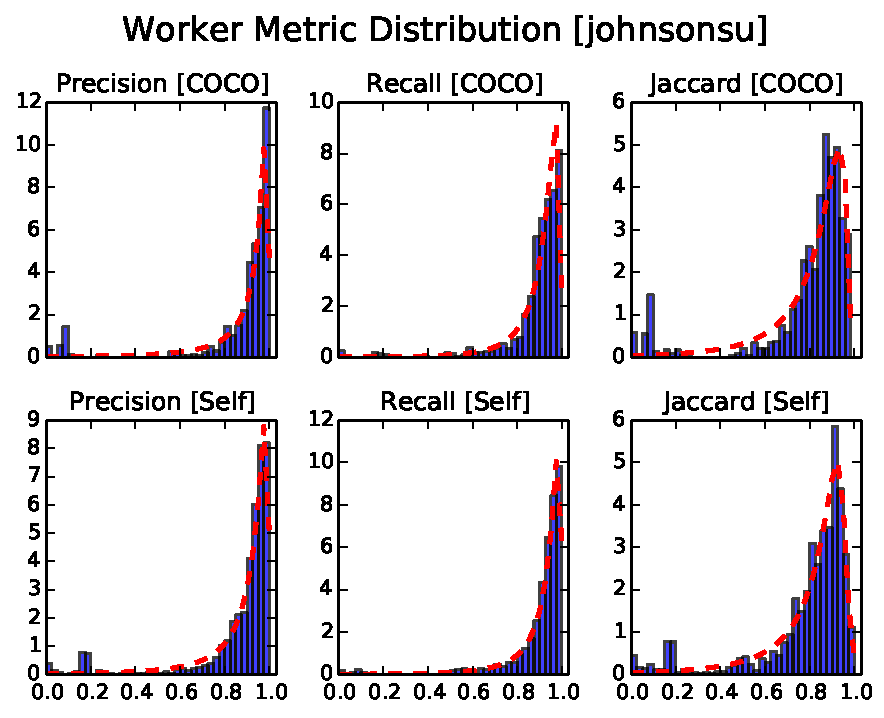
\includegraphics[width=\linewidth]{plots/johnsonsu_fitted_metric_histogram.pdf}
\caption{Normalized histogram of metric values, fitted with a Johnson SU distribution.}
\label{metric_hist}
\end{figure}
\par Overall distribution contains each of the metrics computed from all tasks submitted by all workers (N=1947). The histogram distribution (fixed bin size =50) of these metrics resembles a long-tail, exponential-decaying distribution. As shown in the best-fitting functions in Table \ref{overall_best_fits}, there are many pdfs that fits one metric but not another. 
\par One particular distribution that yields the best fits for many metrics is the Johnson unbounded (SU) distribution, which we summarized in Table \ref{jsu_tbl}. The Johnson SU distribution is a transformed Gaussian where the data $x\mapsto\gamma+\sigma \sinh^{-1}(\frac{x-\xi}{\lambda})$, which effectively maps the typical two-parameter Gaussian to a more flexible, four parameter pdf to better account for the skewness (heavily right-skewed) and kurtosis (long-tail) of the distribution.
\subsection{Object-level Distributions}
\par Recall that $J_i$  is the set of all workers j that annotated the object-image i, we are interested in finding out how these workers are distributed in order to deduce worker quality. 
\par In the data fitting procedure, the bin size is an important hyperparameter. When the bin size is small, the histogram is very smoothed, so many different functional forms can be fitted. Since our data is N=40, we pick a bin size of 30. Due to the large number of $J_i$ distributions, we conducted the fitting procedure on a smaller candidate set of more interpretable functional forms\footnote{Based on our overall function fitting results: Gaussian, Johnson SU/SB, Cauchy, Beta, Loggamma, generalized gamma, Gompertz and t-distributions}.
\par  Table \ref{all_Ji_fit} summarizes the best functional fit for each metric, based on the average RSS across all $J_i$ distributions. The magnitude of RSS for the fitted function of each metric is very different. If we examine a rankings, the RSS difference between the top few best-fit functions is minimal and usually contain the Johnson SU distribution, so the Johnson SU distribution is a sufficiently good description of these $\Phi$ metrics. 
\subsection{Task difficulty Distributions}
We compute the task difficulty according to Eq.\ref{task_difficulty} for all metrics and all objects.  In order to check if the task difficulty agrees with our intuition on which tasks are difficult, we manually labelled our tasks into the three types of errors that workers are prone to make (task ambiguity, small area, and complex boundary)\footnote{Each task can be in more than one category.} We defined the easy tasks as the ones that are neither in any of the error-prone categories, and the overall category contains all 47 tasks.  As shown in Fig.\ref{diff_hist} and Table \ref{di_tbl}, the easy tasks have the lowest average difficulties. Then, of all the error categories, ambiguous tasks makes the task most difficult, followed by hard-to-annotated tasks due to small area and complex boundaries.
\begin{figure}[ht!]
\begin{floatrow}
\ffigbox{%
 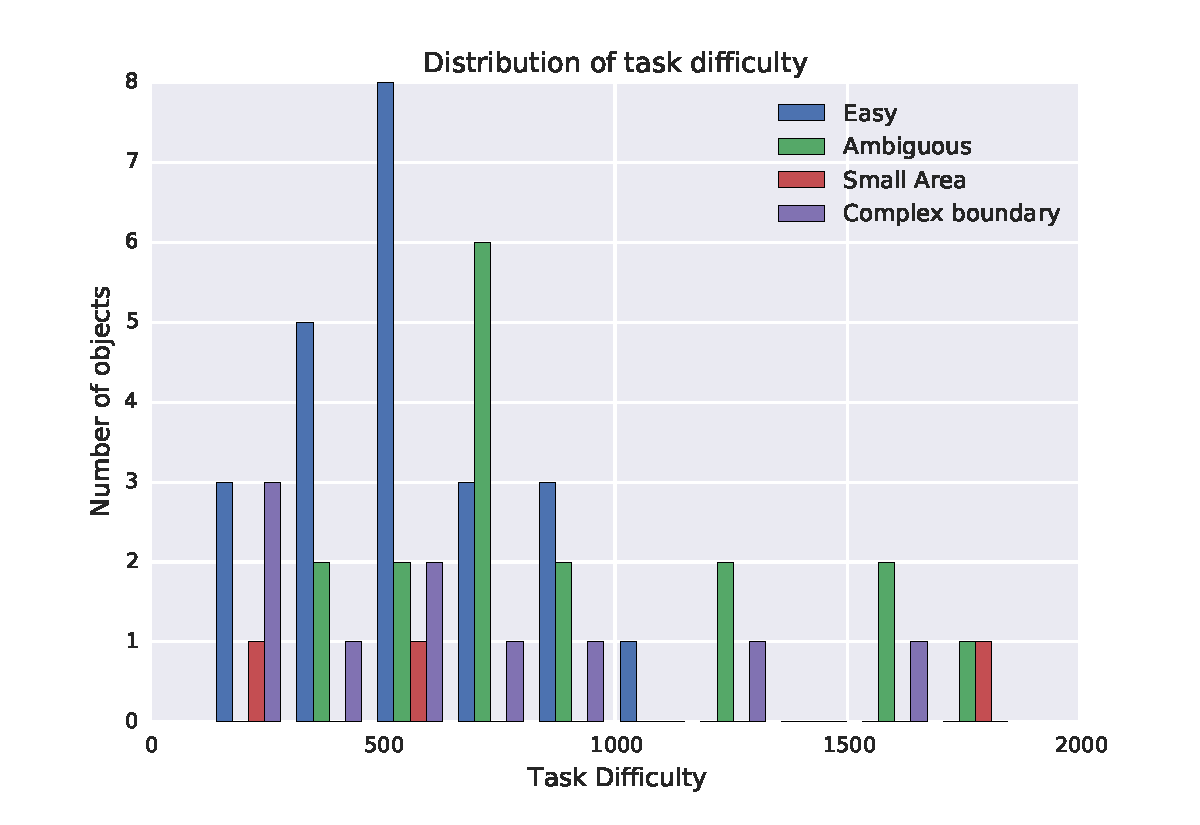
\includegraphics[width=1.1\linewidth]{plots/difficulty_histo.pdf}
}{%
 \caption{The distribution of task difficulty, with bin size of 10.}
 \label{diff_hist}
}
\capbtabbox{%
  \begin{tabular}{lr}
\hline
                  &   Avrg task difficulty \\
\hline
 Easy             &                 565.96 \\
 Overall          &                 655.52 \\
 Complex boundary &                 673.96 \\
 Small area       &                 852.85 \\
 Ambiguous        &                 903.96 \\
\hline
\end{tabular}
}{% 
\caption{Average difficulty per category.}
  \label{di_tbl}
}
\end{floatrow}
\end{figure}


\subsection{Worker Quality Distributions\label{qi_analysis}}
We compute the task difficulty according to Eq.\ref{worker_quality}. We check that users who have high average quality scores often draw erroneous bounding boxes and that workers with low quality scores have consistently accurate bounding boxes\footnote{Note this is opposite from the colloquial notion of ``high-quality`` and ``low-quality``, we can avoid this confusion by transforming the quality score with 1-x or 1/x.}. Fig.\ref{Wqual} shows that the functional form of the worker quality distribution  most resemble a t-distribution.
\begin{figure}[ht!]
\centering
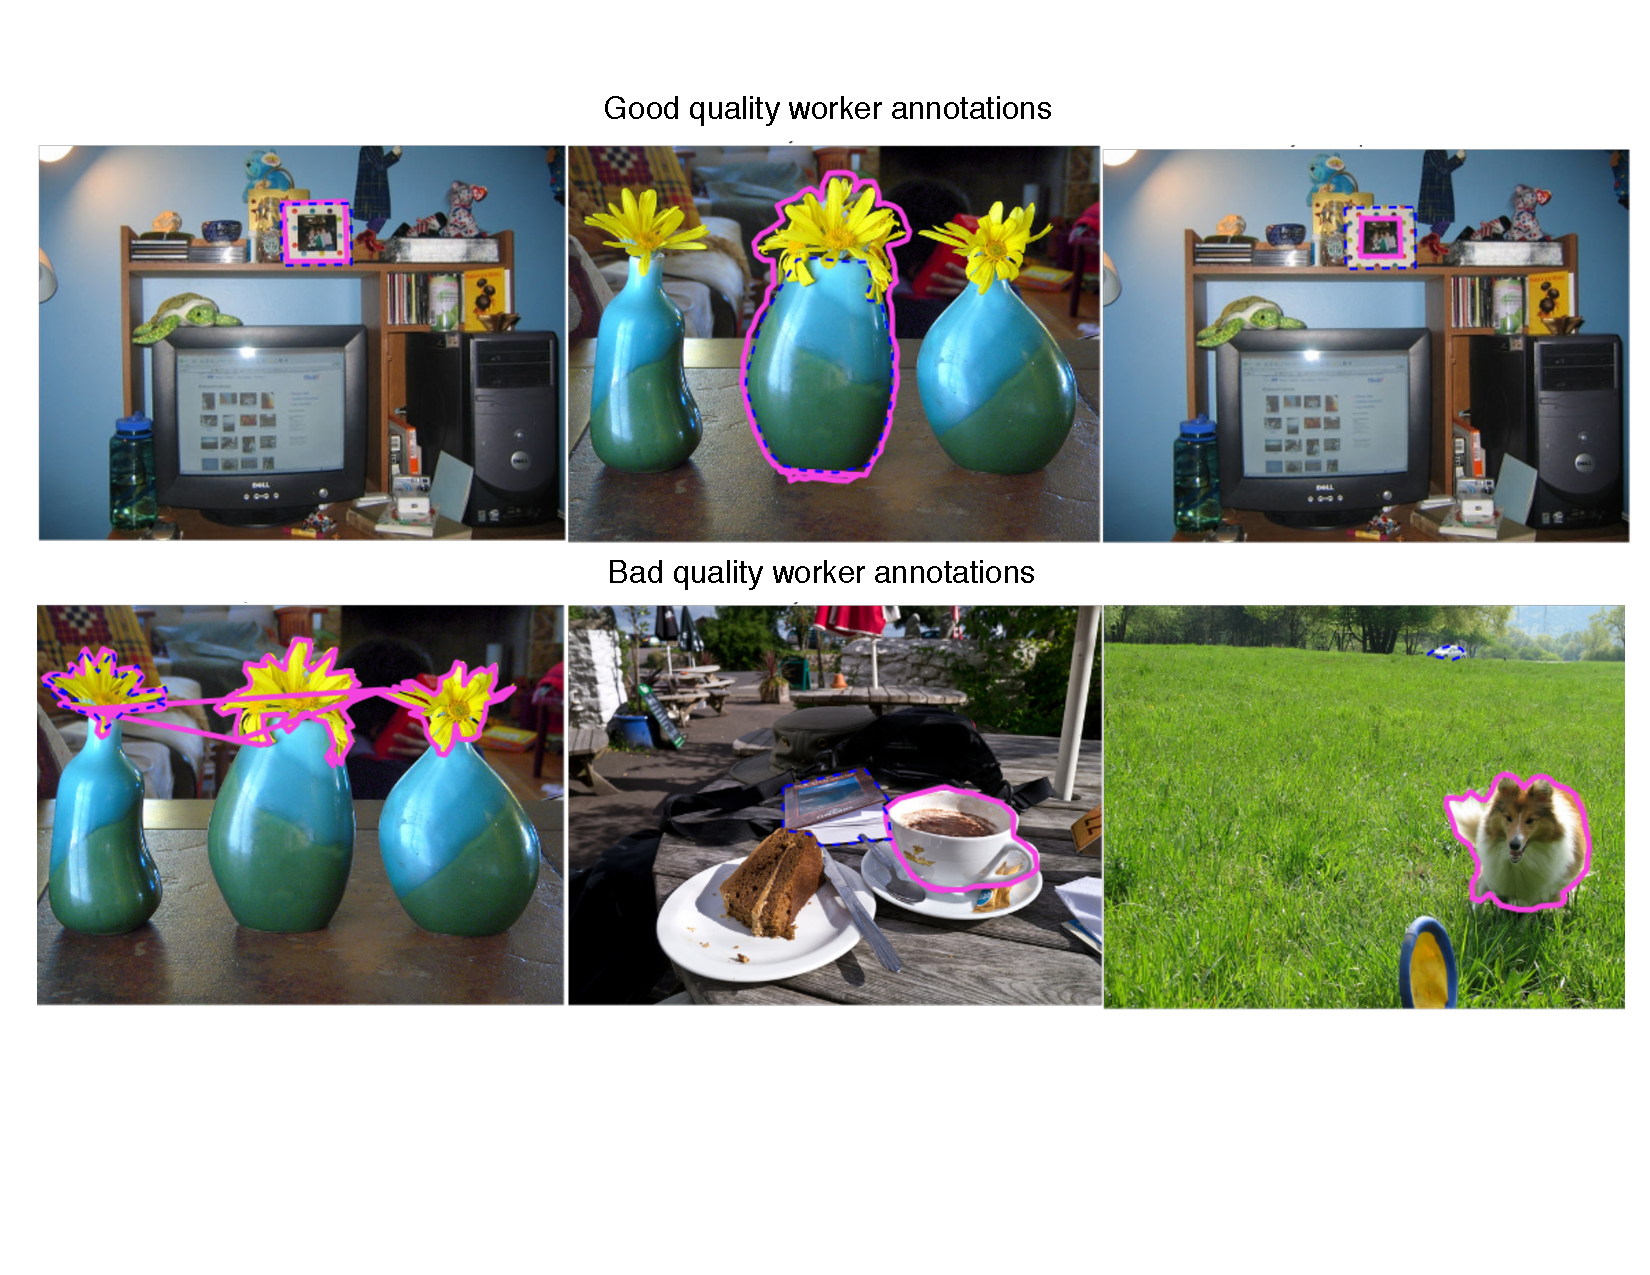
\includegraphics[width=0.9\linewidth]{plots/worker_difficulty.pdf}
\caption{While most of the good quality workers have well-annotated BBs (such as the top left plot), some chosen examples highlights a problematic aspect of using a single metric for measuring work quality from $\phi$ metrics being  incomplete 1-D summaries of the worker's bounding box. For instance, two BB with the same \texttt{NumPts} may resemble very different polygons (top right), and that total recall does not mean that the two bounding box perfectly aligns(top middle). Among the bad workers(bottom middle and right), we have also seen examples where a worker would consistently make the same type of mistake, possibly ignoring the instruction to annotate around the pointed object. }
\end{figure}


\section{Related Works}
\par Despite several large-scale efforts to collect image segmentation from crowds\cite{Lin2014,MartinFTM01,Torralba2010,pascal-voc-2012}, most have relied on simple area-based metrics to quantify their segmentation data quality. Research on quality evaluation of crowd segmentation often make use of heuristic approaches such as quantifying the user types and their clickstream behaviour to determine work quality\cite{Cabezas2015,Sameki2015}. Others have also made use of computer vision features to determine where the annotations should be located, in order to compare against the crowd annotations \cite{Vittayakorn2011,Russakovsky2015}.
\par \citeay{Dawid1979} is the first work that used the EM algorithm to model an individual's biases and skills in the absence of ground truth data, by using a confusion matrix. \citeay{OCWelinder2010} proposes a general model that separately models annotator quality and the biases applied to binary, multivalued and continuous annotations. \citeay{MDWWelinder2010} develops a multidimensional concept of worker qualities and task difficulties by considering object-presence labelling as a noise generation process. The objective truth label is captured by a multidimensional quantity of task-specific measurements and deformed by worker and image related noise, the noisy vector obtained after this process is projected onto the vector of user expertise (which summarizes how well the user percieves each of these measurements), and finally the score is binarized into an inferred label. Many have extended this line of work beyond binary classifications by developing EM-like approaches that works on multiple-choice \cite{Karger2013} as well as free-form responses \cite{Lin2012}. 
\par However, even though EM algorithms assign probabilities regarding  \textit{how good a worker's bounding box is}, for the task of object segmentation, we are ultimately more interested the end goal of \textit{what is the best bounding box that we can get from these data}. Even though the annotation probabilities are sufficient for determining the best binary-labels, image information such as overlapping areas would be useful and not account for in these algorithms. We suspect that this is why many area-based metrics are still more commonly used in practice than EM approaches.
\bibliographystyle{plainnat}
\bibliography{reference}

\newpage
\begin{appendices}
\section{Best-fit summaries}
\begin{table}[ht]
\centering
\begin{tabular}{llrrr}
\hline
 metric           & Function Name   &       RSS &   D-value &   p-value \\
\hline
 Precision [COCO] & beta            &  9.11     &      0.48 &  1.02e-05 \\
 Recall [COCO]    & loggamma        &  4.56     &      0.46 &  2.76e-05 \\
 Jaccard [COCO]   & gompertz        & 13.3      &      0.46 &  2.76e-05 \\
 NME [COCO]       & cauchy          & 51.7      &      0.84 &  1.25e-16 \\
 Num Points       & johnsonsb       &  0.000239 &      1    &  2.16e-23 \\
 Precision [Self] & johnsonsu       &  6.02     &      0.34 &  0.00443  \\
 Recall [Self]    & johnsonsu       &  5.07     &      0.42 &  0.000178 \\
 Jaccard [Self]   & johnsonsu       &  4.57     &      0.28 &  0.0317   \\
 NME [Self]       & johnsonsb       & 30.3      &      0.74 &  5.31e-13 \\
 Area Ratio       & gengamma        & 27.1      &      0.34 &  0.00443  \\
\hline
\end{tabular}
\caption{Shapewise, the RSS is a better measure of functional fit than p-value, so we use this for evaluating the best-fitting pdf for each measure. This table summarizes the best-fitting function for each metric.}
\label{overall_best_fits}
\end{table}

\begin{table}[ht]
\centering
\begin{tabular}{lrrrrrrr}
\hline
 metric           &      RSS &   D-value &   p-value &   $\xi$ &   $\lambda$ &   Shift &   Scale \\
\hline
 Precision [COCO] & 10       &      0.36 &   0.0021  &  5.2 &     0.75 &  1      & 0.00011 \\
 Recall [COCO]    &  7       &      0.44 &   7.2e-05 &  5.9 &     1.1  &  1      & 0.00062 \\
 Jaccard [COCO]   & 14       &      0.3  &   0.017   &  5.6 &     1.1  &  0.99   & 0.0017  \\
 NME [COCO]       &  2.2e+02 &      0.7  &   1.1e-11 &  1.3 &     0.61 &  0.99   & 0.0032  \\
 Num Points       &  0.00044 &      1    &   2.2e-23 & -6.2 &     1.2  &  0.8    & 0.21    \\
 Precision [Self] &  6.8     &      0.34 &   0.0044  &  5.6 &     0.84 &  1      & 0.00018 \\
 Recall [Self]    &  5.5     &      0.42 &   0.00018 &  5.5 &     0.91 &  1      & 0.00029 \\
 Jaccard [Self]   &  4.6     &      0.28 &   0.032   &  1.6 &     0.95 &  0.96   & 0.039   \\
 NME [Self]       &  1.1e+02 &      0.64 &   7.8e-10 &  1.2 &     0.61 &  0.99   & 0.0037  \\
 Area Ratio       & 30       &      0.32 &   0.0089  & -4.9 &     0.78 & -0.0002 & 0.00012 \\
\hline
\end{tabular}
\caption{Johnson SU fitting coefficients.}
\label{jsu_tbl}
\end{table}

\begin{table}[ht]
\centering
\begin{tabular}{llr}
\hline
 metric           & Function   &       RSS \\
\hline
 Area Ratio       & johnsonsu  & 273751.49 \\
 Jaccard [COCO]   & johnsonsu  &    675.65 \\
 Jaccard [Self]   & cauchy     &    250.42 \\
 NME [COCO]       & johnsonsu  &  27439.87 \\
 NME [Self]       & johnsonsu  &  10812.98 \\
 Num Points       & cauchy     &      0.06 \\
 Precision [COCO] & johnsonsu  &   4570.24 \\
 Precision [Self] & johnsonsu  &   1414.98 \\
 Recall [COCO]    & johnsonsu  &    452.79 \\
 Recall [Self]    & beta       &    902.61 \\
\hline
\end{tabular}
\caption{Best functional fit for each metric, as determined by average RSS across all objects in the $J_i$ distribution.}
\label{all_Ji_fit}
\end{table}
\begin{table}[ht]
\centering
\begin{tabular}{lrrrrrrrrrr}
\hline
          &   P [C] &   R [C] &   J [C] &   NME [C] &   NumPt &   P [C] &   R [S] &   J [S] &   NME [S] &   Area \\
\hline
 R [Norm] &    0.05 &   -0.27 &   -0.11 &      0.32 &    0.84 &    0.18 &   -0.36 &   -0.05 &      0.27 &   0.60 \\
 p[Norm]  &    0.85 &    0.30 &    0.67 &      0.22 &    0.00 &    0.49 &    0.15 &    0.87 &      0.29 &   0.01 \\
 R [JSU]  &    0.31 &    0.02 &    0.03 &     -0.12 &   -0.26 &    0.47 &   -0.19 &    0.61 &      0.51 &   0.27 \\
 p [JSU]  &    0.22 &    0.95 &    0.90 &      0.64 &    0.31 &    0.05 &    0.47 &    0.01 &      0.04 &   0.29 \\
\hline
\end{tabular}
\caption{Pearson's linear correlation coefficient when comparing the average number of points in BB drawn by all worker(as an indicator for task difficulty) and the standard deviation of the worker distribution (against \texttt{JSU} and \texttt{Norm} distributions). [C],[S] short for [COCO] and [Self].}
\label{assum3}
\end{table}
\newpage
\section{Data Preprocessing}
\par In order to compute Euclidean distances scores and normalize the input coordinates to the EM algorithm, we conduct the two step procedure to preprocess the worker's responses. First, we interpolate the user's bounding box to a larger set of points, so that the set of coordinates described by worker's bounding box are of the same length  (m=50). Then, we align these points so that the list of coordinates starts from the left most side of the polygon in a counterclockwise manner. This alignment procedure ensures that we are making a fair comparison between the different worker's bounding boxes. 
\par For the sampling stage, we attempted at two different approaches: B-spline parametric interpolation and random-walk sampling. We found that the results of B-spline interpolation can significantly distort the shape of the bounding boxes when the number of control points is low, as shown in Fig.\ref{interpolation}.
\begin{figure}[ht!]
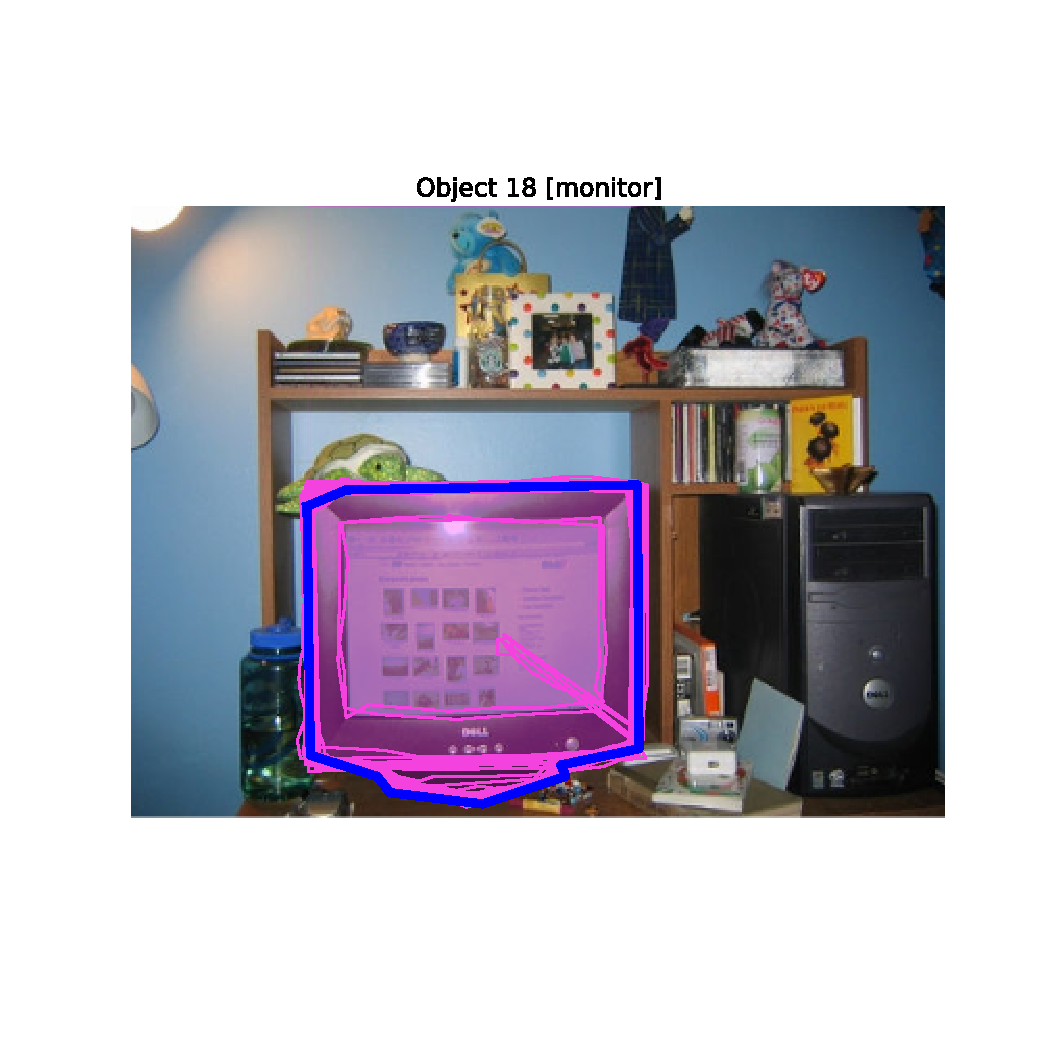
\includegraphics[width=0.3\linewidth]{plots/bb_object_18.pdf}
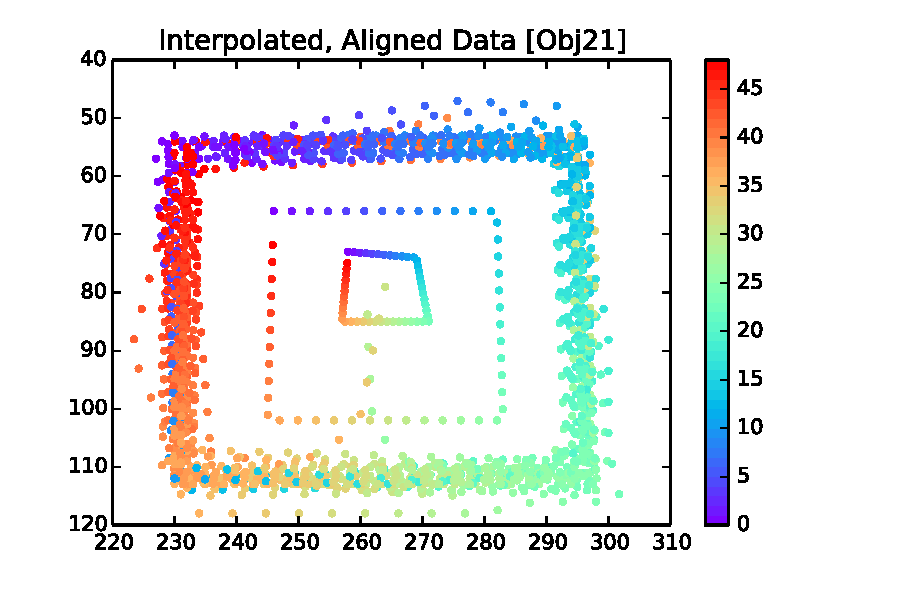
\includegraphics[width=0.3\linewidth]{plots/random_interpolated_aligned.pdf}
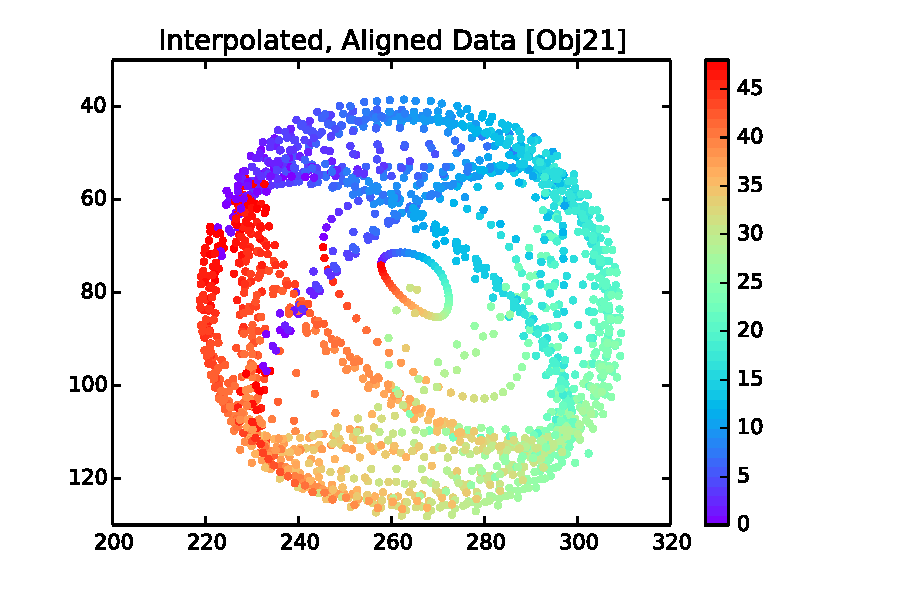
\includegraphics[width=0.3\linewidth]{plots/bspline_interpolated_aligned.pdf}
\caption{Interpolation based on the random walk technique (center) versus the spline interpolation technique(left).}
\label{interpolation}
\end{figure}
\par For bounding box alignment, our implementation differs slightly from the one in  \cite{Vittayakorn2011} in that we do not use the Munkres algorithm for BB alignment. The Munkres algorithm is a combinatorial optimization that tries to find lowest-cost (pairwise distances) sets of two given bounding boxes, but since we know that all control poitns on the bounding box is drawn sequentially, we can use a simpler algorithm. Our alignment procedure first identifies the control point closest to the origin. Then we test neighboring control points to determine whether the bounding box was drawn in the clockwise or counter-clockwise fashion, in order to generate the resulting aligned bounding box. This alignment procedure has two advantages over the Munkres algorithm: 1) it significantly decreases the amount of pairwise distances that needs to be computed so this approach is less computationally-demanding and 2) it aligns the bounding box against a global image orgin rather than against a ground truth bounding box, which may vary for every object \footnote{This is important for EM but not for Euclidean distance calculation}. 
\begin{figure}[ht!]
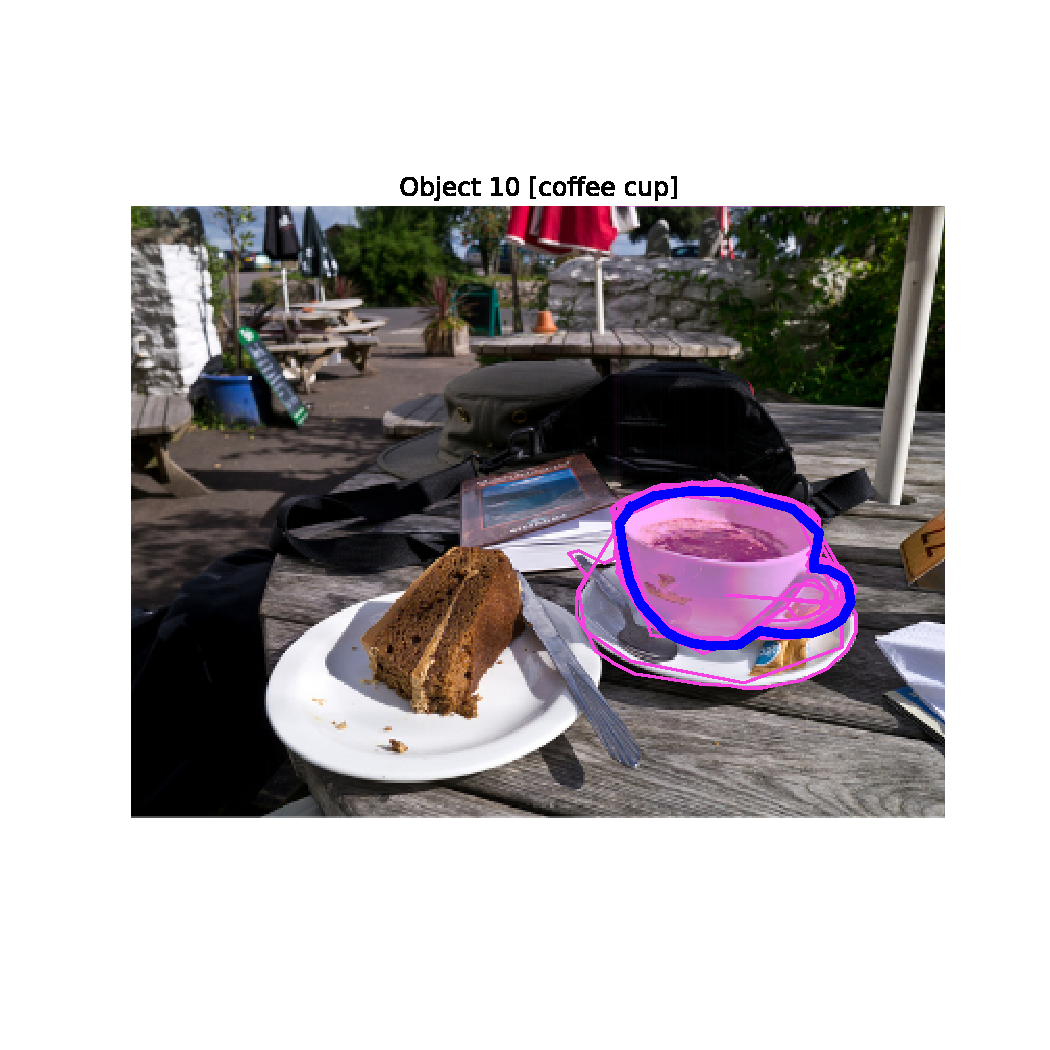
\includegraphics[width=0.24\linewidth]{plots/bb_object_10.pdf}
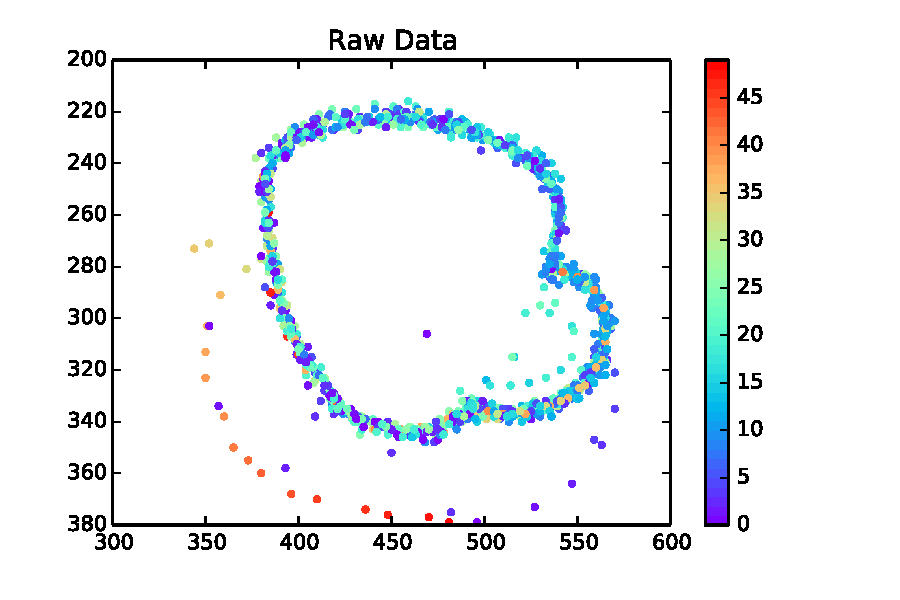
\includegraphics[width=0.24\linewidth]{plots/raw_data.pdf}
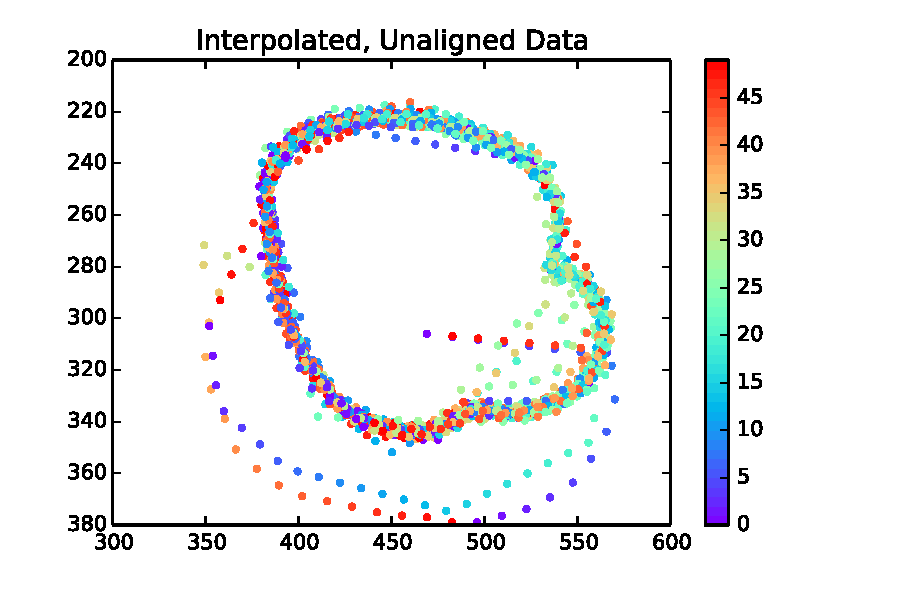
\includegraphics[width=0.24\linewidth]{plots/interpolated_unaligned_data.pdf}
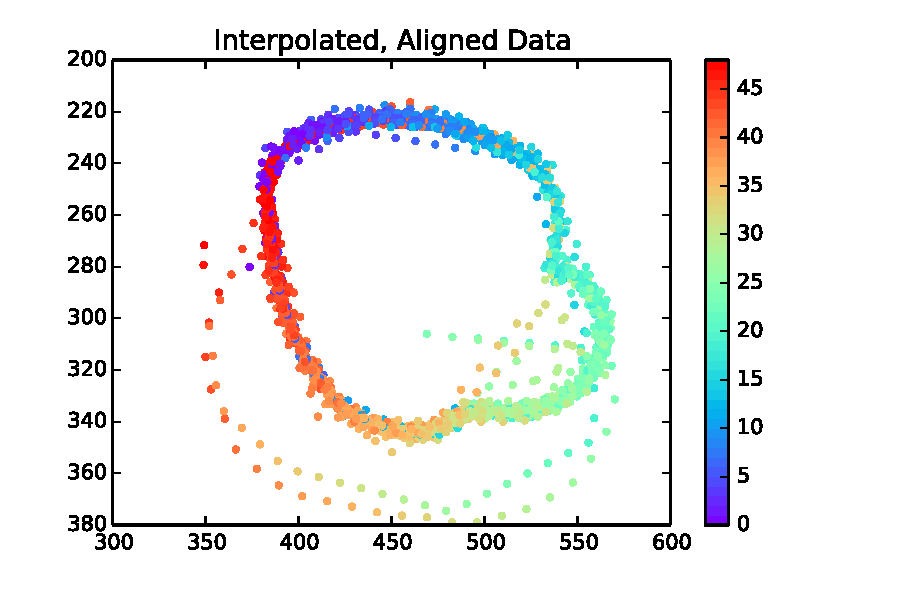
\includegraphics[width=0.24\linewidth]{plots/interpolated_aligned_data.pdf}
\label{result}
\caption{Top left  : Bounding box from all workers  of the coffee cup. Top right: The control point colors indicate the index of point in the set of coordinates of that bounding box. The uninterpolated data shows that the average worker draws up to about 25 points for each bounding box. Bottom left: We interpolate the bounding boxes to 50 control points. Bottom right: The bounding boxes are aligned from the origin starting at the top left corner and proceeding in a clockwise fashion.}
\end{figure}

\section{Additional Plots}
Visualizations for all the object annotations could be found \href{http://nbviewer.jupyter.org/github/dorisjlee/crowd-seg/blob/master/analysis/2017_01_16_Visualize_all_bb_results.ipynb}{here}.
\begin{figure}[ht!]
\centering
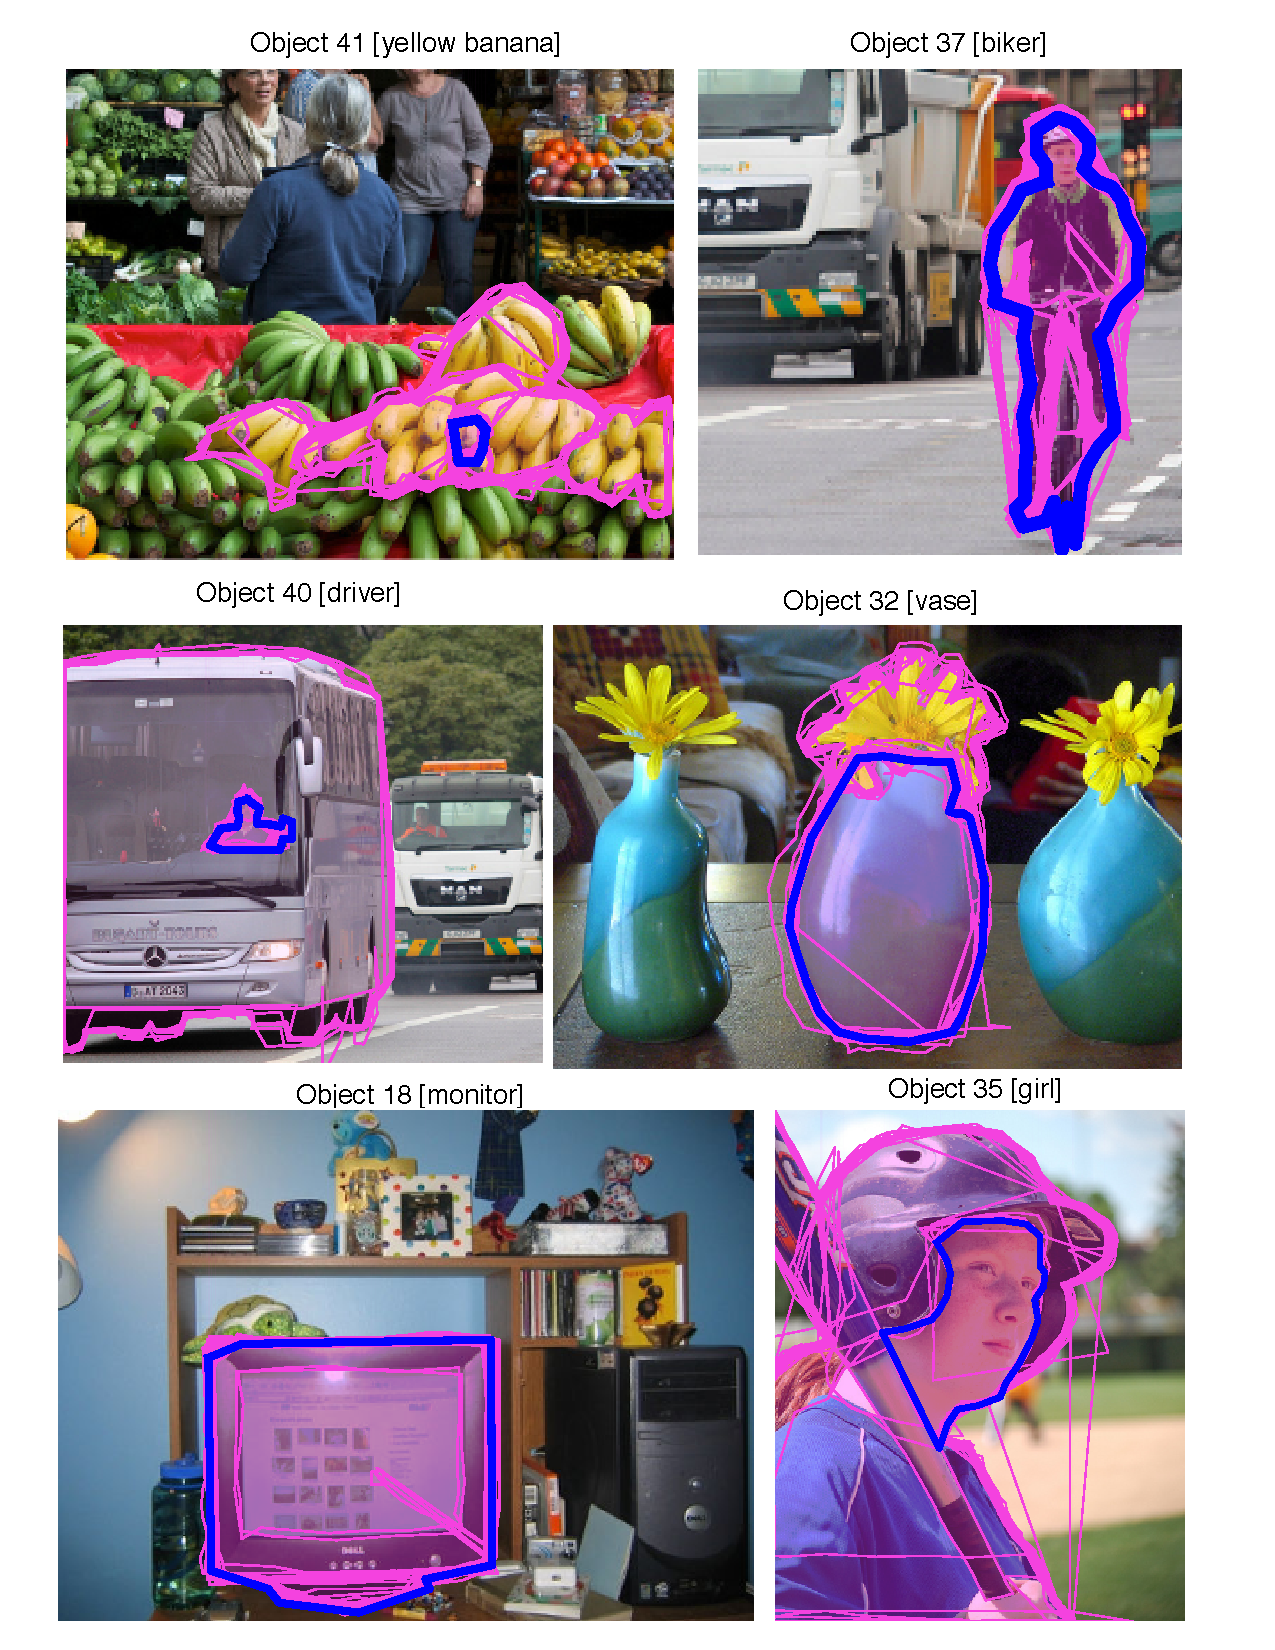
\includegraphics[width=\linewidth]{plots/task_ambiguous_cases.pdf}
\caption{Selected task ambiguous object that is excluded in the task difficulty analysis. }
\end{figure}
\begin{figure}[ht!]
\centering
\fbox{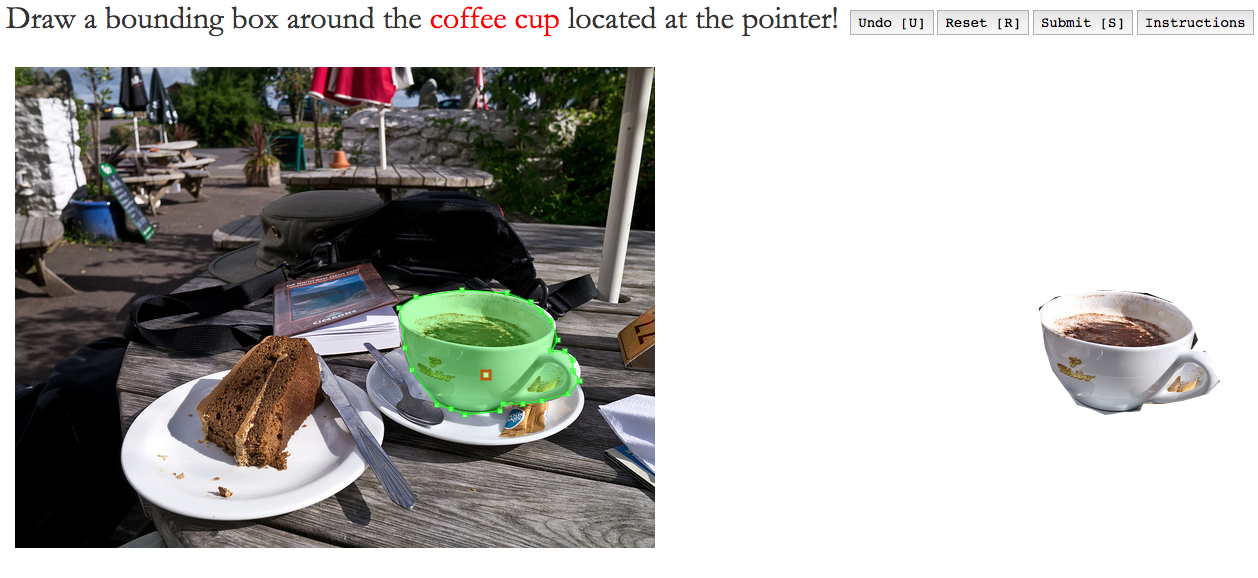
\includegraphics[width=0.9\linewidth]{plots/interface.png}}
\caption{An example interface for the segmentation webapp can be seen  \href{http://crowd-segment.herokuapp.com/segment/COCO_train2014_000000000127/10/}{here}.}
\label{interface}
\end{figure}
% Fig.\ref{qvsqplot} also shows that, in general, the more task accomplished by the worker, the better the quality of their work, which suggests potential learning effects of the task. 
\begin{figure}[ht]
\centering
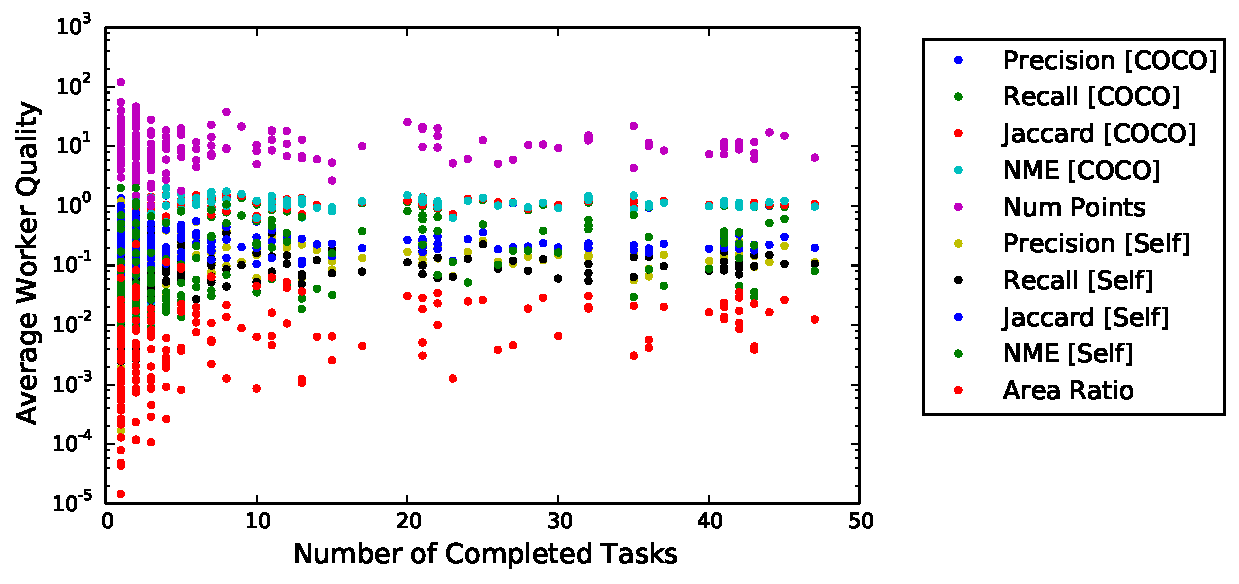
\includegraphics[width=0.9\linewidth]{plots/quality_vs_quantity.pdf}
\caption{ When a worker completes many tasks, their work quality is fairly good on average(Right region of plot). If the worker only completes a few tasks, they can either draw one very good bounding box (Bottom left), or they may draw a really bad one(Top left). In the small number of tasks case, the spread in work quality is large. }
\label{qvsqplot}
\end{figure}

\begin{figure}[ht!]
\centering
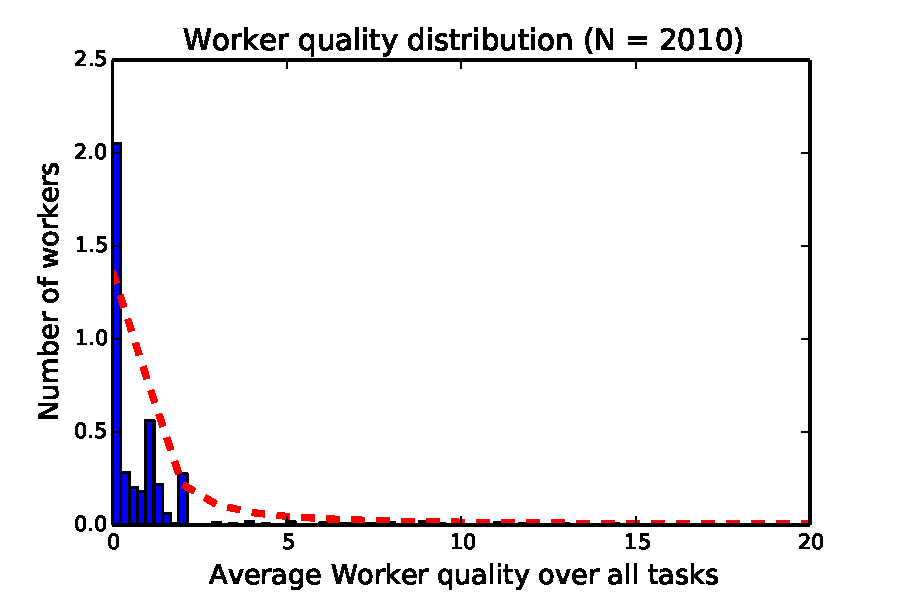
\includegraphics[width=0.8\linewidth]{plots/Wqual_dist.pdf}
\caption{The normalized histogram with bin size of 500 fits best to a t-distribution, with RSS of 0.38. These trends are simmilar to the results in Figure 6c of \cite{OCWelinder2010}.}
\label{Wqual}
\end{figure}


\end{appendices}
\end{document}
%%%%%%%%%%%%%%%%%%%%%%%%%%%%%%%%%%%%%%%%%%%%%%
%%%%%%%%%%%%%%%%%%%%%%%%%%%%%%%%%%%%%%%%%%%%%%
%%%%%%%%%%%%%%%%%%        SCRAP         %%%%%%%%%%%%%%%%%% 
%%%%%%%%%%%%%%%%%%%%%%%%%%%%%%%%%%%%%%%%%%%%%%
%%%%%%%%%%%%%%%%%%%%%%%%%%%%%%%%%%%%%%%%%%%%%%


%\begin{itemize}
%\item Alternatively, we can also model $q_{ij}$ as a random variable drawn from a distribution. Since the task difficulty and worker quality does not  completely determine the quality of bounding box that a worker would draw next. Therefore, the distribution of $\phi_{ij}$ given a new bounding box $z_{j}$ can be described as:
%\begin{equation}
%p(\phi_{ij}|z_{j}) = f(\phi_i;q_{j'},D_i)
%\end{equation}
%where $j'$ includes all object labelled by worker j up to object i.
%\end{itemize}
% how the worker performs historically$q_{j'}$
%is determined by both the objective description of $z_i$
% and the difficulty of the task. 
%Here, we can model the distribution of $\phi_i$ as :
%$$p(\phi_i|z_i) = N(\phi_i;z_i,D_i^2)$$



%\par Many of the best-fitting functional form of $\Phi$ in Table \ref{all_Ji_fit} may make the inference problem challenging. While the Gaussian does not yield the best fit, it is a more interpretable $\Phi$ function and may be easier for inference. Some of the non-Gaussianity may also be due to the small sample size in our preliminary experiment (N$\approx$40 for each $J_i$ distribution). We are interested in assessing whether it can be a ``good-enough'' fit based on RSS. 
%\par  Fig.\ref{GaussRSSBox} shows a boxplot of the RSS based on the Gaussian fits for all the $J_i$ distributions. We could see that the number of control points have several orders of magnitude lower RSS than other metrics. This makes sense because \texttt{Num Points} is the only metric that measures \textit{only} how carefully drawn the BB is, which would in theory match with a spread in worker dexterity. All other metrics (except \texttt{Area Ratio}) are confounded by potential BB mismatch or task ambiguity mistakes because of normalization or comparison against a gold standard BB. 
%\begin{figure}[ht]
%\centering
%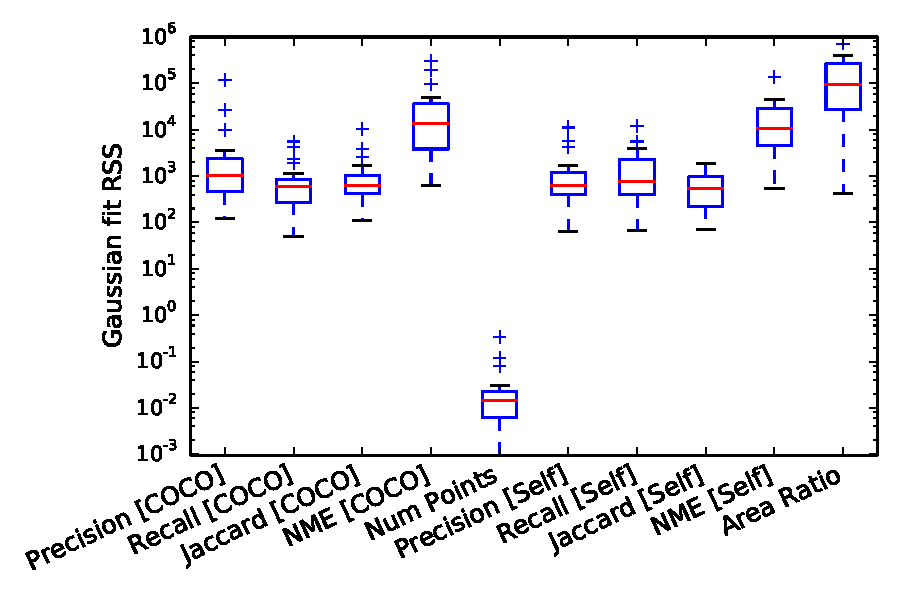
\includegraphics[width=0.6\linewidth]{plots/GaussianRSSBoxplot.pdf}
%\caption{The boxplot shows the spread of RSS for all $J_i$ distribution based on Gaussian fits.}
%\label{GaussRSSBox}
%\end{figure}
%\subsubsection{Testing Assumption 3: Influence of task difficulty on spread}
%We are interested in testing our hypothesis that if work quality exhibits a large spread, that means that the object i is probably very hard to annotate. If we exclude difficult task due to task ambiguity, we hypothesize that the number of points in the image object (as a measure of boundary complexity) should depend on the standard deviation of the fitted distribution (Gaussian or Johnson SU). As summarized in Table \ref{assum3}, the Pearson's test shows that there is \textit{very little evidence for linear correlation} between the number of points in an object and the standard deviation of the fitted function. One potential reason for this is that the number of points is not a good metric of task difficulty, since we know that there are other types of error that could make a task difficult (small object area and task ambiguity) A potential next step would be to look at how the data for selected object subpopulations that are prone to each errors type would behave, but due to the small number of objects in each category the results for this analysis will probably not be very generalizable. 

%\subsubsection{Testing Assumption 2: }
%Since our metrics are all 
%ground truth means that --- as 1. So effectively, we are measuring 1-f(x) 
%\item We are interested in whether our data agrees with Assumption \#2 and \#3 regarding work quality and task difficulty. 
%If a worker's response differs greatly from the ground truth, then work quality ($Q_w$) is low. 
%If many of the worker's response differs greatly from ground truth for a particular image, then task difficulty ($D_t$) is high.
